\graphicspath{{2groups/asy/}}

\section{Groups: Axioms and Basic Examples}\label{chap:groups}

In this chapter we define our main objects of study and introduce some of the vocabulary and examples used throughout the course---the ``Key concepts/definitions'' listed at the start of each Exercise set. Most examples are very simple; their purpose is to help make sense of the abstract ideas. If an example seems too confusing, feel free to ignore it on first reading! 


\subsection{The Axioms of a Group}\label{sec:groupaxioms}

\begin{defn}{Closure}{}
A \emph{binary operation} $*$ on a set $G$ is a function $*:G\times G\to G$. Equivalently,
\[
	\forall x,y\in G,\text{ we have }x\opast y\in G\tag{$\dag$}
\]
We say that $G$ is \emph{closed} under $*$, and that $(G,*)$ is a \emph{binary structure.}
\end{defn}


In abstract situations (including most theorems) we typically drop the $\ast$ symbol and use \emph{juxtaposition} ($x\opast y=xy$). However, in explicit \emph{examples} this might be a bad idea, say if $*$ is addition\ldots

\begin{examples}{}{basicexs}
	\exstart Addition ($+$) is a binary operation on the set of \emph{integers} $\Z$:\vspace{-2pt}
	\begin{enumerate}\setcounter{enumi}{1}\itemsep2pt
		\item[]\begin{quote}
			Given $x,y\in\Z$, we know that $x+y\in\Z$
		\end{quote}
		\smallskip
		This isn't a claim you can \emph{prove}, since it is really part of the \emph{definition} of integer addition.

	  \item Subtraction ($-$) is \emph{not} a binary operation on the positive integers $\N=\{1,2,3,4,\ldots\}$. This you can prove; to show that ($\dag$) is \emph{false,} exhibit a \emph{counter-example}
	  \[
	  	1-7=-6\not\in\N\tag{$\exists x,y\in\N$ such that $x-y\not\in\N$}
	  \]
	  On the integers, however, subtraction is a binary operation: $\Z$ is closed under $+$.
  
  %\item Division ($\div$) is \emph{not} a binary operation on $\Z$: for instance $2\div 3=\frac 23\not\in\Z$. Division is a binary operation on the set $\R^\times$ of \emph{non-zero} real numbers.
  
	 	\begin{minipage}[t]{0.79\linewidth}\vspace{0pt}
		  \item\label{ex:table1} On a small set, it can be convenient to use a table to represent a binary operation. The given table describes an operation on a set of three elements $\{e,a,b\}$. Read the  \emph{left} column first, then the \emph{top} row: for instance,
		  \[
		  	\textcolor{red}{a}\textcolor{blue}{b}=\textcolor{Green}{e}
		  \]
		\end{minipage}
		\hfill
		\begin{minipage}[t]{0.2\linewidth}\vspace{0pt}
			\flushright
			$\begin{array}{c||c|c|c}
				* & e & a & \textcolor{blue}{b}\\\hline\hline
				e & e & a & b\\\hline
				\textcolor{red}{a} & a & e & \textcolor{Green}{e}\\\hline
				b & b & e & a
			\end{array}$
		\end{minipage}
	\end{enumerate}
\end{examples}

We'll continue checking these examples for each of the remaining axioms.


\begin{defn}{Associativity}{assoc}
	A binary structure $(G,\ast)$ is \emph{associative} if
	\[
		\forall x,y,z\in G,\quad x(yz)=(xy)z
	\]
	If $\ast$ is associative, then the expression $x y z$ has unambiguous meaning, as does the usual \emph{exponential/power} notation shorthand, e.g.\ $x^n=x\cdots x$.
\end{defn}


\begin{examples*}{\ref{ex:basicexs}, ver.\,II}{}
	\exstart Addition is associative: $x+(y+z)=(x+y)+z$ for any integers.\vspace{-2pt}
	\begin{enumerate}\setcounter{enumi}{1}\itemsep2pt
	  \item $(\Z,-)$ is non-associative: e.g.\ $(1-1)-2=-2\neq 2=1-(1-2)$.
	  %\item $(\R^\times,\div)$ is non-associative: e.g.\ $2\div(4\div 2)=\frac 2{4/2}=1\neq \frac 18=\frac{2/4}2=(2\div 4)\div 2$.
	  \item $\bigl(\{e,a,b\},*\bigr)$ is non-associative: e.g.\ $a(b^2)=a^2=e\neq b=eb=(ab)b$.
	\end{enumerate}
\end{examples*}

\goodbreak

\begin{defn}{Identity}{}
	A binary structure $(G,\ast)$ has an \emph{identity element} $e\in G$ if
	\[
		\forall x\in G,\quad ex=xe=x
	\]
\end{defn}

\begin{examples*}{\ref{ex:basicexs}, ver.\,III}{}
	\exstart Addition on $\Z$ has identity 0, since $0+x=x+0=x$ for any integer $x$.
	\begin{enumerate}\setcounter{enumi}{1}\itemsep2pt
	  \item $(\Z,-)$ does not have an identity: e.g.\ if $e-x=x$, then $e=-2x$ would depend on $x$!
	  %\item $(\R^\times,\div)$ does not have an identity: $e\div x=\frac ex=x\implies e=x^2$ again depends on $x$.
	  \item $\bigl(\{e,a,b\},*\bigr)$ has identity $e$; observe the first row and column of the table.
	\end{enumerate}
\end{examples*}

By convention, if $G$ is finite and has an identity (e.g.\ Example \ref*{ex:basicexs}.\ref{ex:table1},) we list it first. Indeed, we can always list \emph{it} first, since\ldots

\begin{lemm}{Uniqueness of identity}{}
	A binary structure $(G,\ast)$ has at most one identity.
\end{lemm}

It is now legitimate to refer to \emph{the} identity $e$. Uniqueness proofs in mathematics often follow a standard pattern: suppose there are two such objects and show that they are identical.

\begin{proof}
	Suppose $e,f\in G$ are identities. Then
	\[
		ef=
		\begin{cases}
			f&\text{since $e$ is an identity}\\
			e&\text{since $f$ is an identity}
		\end{cases}
	\]
	Since $f=e$, there is only one identity.
\end{proof}

We used almost nothing about $(G,*)$; in particular it need not be associative (e.g.\ Example \ref*{ex:basicexs}.\ref{ex:table1}).

\begin{defn}{Inverse}{}
	Let $(G,*)$ have identity $e$. An element $x\in G$ has an \emph{inverse} $y\in G$ if
	\[
		xy=yx=e
	\]
\end{defn}

\begin{examples*}{\ref{ex:basicexs}, ver.\,IV}{}
	\exstart Every integer $x$ has an inverse under addition: $x+(-x)=(-x)+x=0$.\vspace{0pt}
	\begin{enumerate}\setcounter{enumi}{1}\itemsep2pt
	  \item Since $(\Z,-)$ has no identity, the question of inverses makes no sense.
	  
	  \begin{minipage}[t]{0.7\linewidth}\vspace{-2pt}
	  	\item Since $e^2=a^2=ab=ba=e$, we see that every element has an inverse; indeed $a$ has \emph{two} inverses!
	  \end{minipage}
	  \hfill
	  \begin{minipage}[t]{0.29\linewidth}\vspace{-2pt}
		  \flushright
		  $\begin{array}{l||c|c|c}
		  	\text{Element}&e&a&b\\\hline
		  	\text{Inverse(s)}&e&a,b&a
		  \end{array}$
	  \end{minipage}
	\end{enumerate}
\end{examples*}



\begin{lemm}{Uniqueness of inverses}{uniqueinv}
Suppose $(G,\ast)$ is associative and has an identity. If $x\in G$ has an inverse, then it is unique.
\end{lemm}

\begin{proof}
Suppose $x$ has inverses $y,z\in G$. Then,
\[
	z(\textcolor{red}{xy})=(\textcolor{blue}{zx})y \implies z\textcolor{red}{e}=\textcolor{blue}{e}y \implies z=y
	\tag*{\qedhere}
\]
\end{proof}

Note where associativity was used in the proof. Example \ref*{ex:basicexs}.\ref{ex:table1} shows that this condition is \emph{necessary}: a non-associative structure can have non-unique inverses.

\goodbreak

\begin{defn}{Commutativity}{}
	Let $(G,*)$ be a binary structure. Elements $x,y\in G$ \emph{commute} if $xy=yx$. We say that $*$ is \emph{commutative} if all elements commute:\vspace{-3pt}
	\[
		\forall x,y\in G,\ xy=yx
	\]
\end{defn}


\begin{examples*}{\ref{ex:basicexs}, ver.V}{}
	\exstart Addition of integers is commutative: $\forall x,y\in\Z$, $x+y=y+x$.\vspace{-3pt}
	\begin{enumerate}\setcounter{enumi}{1}\itemsep0pt
	  \item Subtraction of integers is \emph{non-commutative}: e.g.\ $2-3\neq 3-2$.
	  %\item Division is non-commutative: e.g.\ $\frac 23\neq 3\frac 32$.
	  \item The relation is commutative since its table is \emph{symmetric} across its main $\searrow$ diagonal.
	\end{enumerate}
\end{examples*}

To obtain our main definition, simply assemble the pieces!

\begin{defn}{Group axioms}{group}
	A \emph{group} $G$ is a binary structure $(G,*)$ satisfying the \emph{associativity} and \emph{identity} axioms, and for which all elements have \emph{inverses.} This is summarized by the mnemonic\vspace{-2pt}
	\begin{quote}
		\emph{Closure, Associativity, Identity, Inverse}\vspace{-2pt}
	\end{quote}
	The \emph{order} of $G$ is its cardinality $\nm G$.
	Moreover, $G$ is \emph{abelian} if $*$ is \emph{commutative.}
\end{defn}

Of our examples, only $(\Z,+)$ is a group; indeed an \emph{abelian, infinite order, additive\footnote{\label{fn:additive}The operation is addition; a \emph{multiplicative} group follows the multiplication/juxtaposition convention. These are distinctions only of notation: e.g.\ $x+x+x=3x$ in an additive group corresponds to $xxx=x^3$ in a multiplicative group.}} group. The same observations show that $(\Q,+)$, $(\R,+)$ and $(\C,+)$ are abelian groups.\par

While it is common practice to refer to a set $G$ as a group, you should do so \emph{only if the operation $\ast$ is obvious to everyone}. Writing ``$\Z$ is a group \emph{under addition},'' is much safer than ``$\Z$ is a group.''

\begin{examples}{}{rx}
	\exstart The non-zero real numbers $\R^\times$ form an abelian group under multiplication.\vspace{-5pt}
	\begin{enumerate}\setcounter{enumi}{1}\itemsep0pt
	  \item[]\begin{quote}\renewcommand{\arraystretch}{1.1}
			\begin{tabular}{@{}ll}
				\emph{Closure}&If $x,y\neq 0$, then $xy\neq 0$\\
				\emph{Associativity}&$\forall x,y,z,\ x(yz)=(xy)z$\\
				\emph{Identity}&If $x\neq 0$, then $1\cdot x=x\cdot 1=x$, so $1\in\R^\times$ is an identity\\
				\emph{Inverse}&Given $x\neq 0$, observe that $x^{-1}=\frac 1x$ is an inverse: $x\cdot \frac 1x=\frac 1x\cdot x=1$\\
				\emph{Commutativity}&If $x,y\neq 0$, then $xy=yx$
			\end{tabular}
		\end{quote}
		As before, we cannot prove these claims since they are part of the definition of multiplication.	Similarly, $(\Q^\times,\cdot)$ and $(\C^\times,\cdot)$ are abelian groups.
		
		  
	  \item The \emph{even} integers $2\Z=\{2z:z\in\Z\}$ form an abelian group under addition.
	%   \begin{quote}
	% 	\renewcommand{\arraystretch}{1.2}
	% 	\begin{tabular}{@{}ll}
	% 		\emph{Closure}&If $2x,2y\in 2\Z$, then $2x+2y=2(x+y)\in 2\Z$\\
	% 		\emph{Associativity}&If $2x,2y,2z\in 2\Z$, then $2x(2y\cdot 2z)=8xyz=(2x\cdot 2y)\cdot 2z$\\
	% 		\emph{Identity}&$0=2\cdot 0\in 2\Z$ is the additive identity\\
	% 		\emph{Inverse}&$2x$ has inverse $-2x=2(-x)\in 2\Z$: indeed $2x+2(-x)=0=2(-x)+2x$\\
	% 		\emph{Commutativity}&$2x+2y=2y+2x$
	% 	\end{tabular}
	% 	\end{quote}
		%Indeed the same is true for $n\Z=\{nz:z\in\Z\}$ and any constant $n\in\R$ (Exercise \ref{exs:nzgroup}).
	  
	  \item The \emph{odd} integers $1+2\Z=\{1+2n:n\in\Z\}$ do not form a group under addition since they are not closed: for instance, $1+1=2\not\in 1+2\Z$.
	  
	  \item Every vector space is an abelian group under addition. %This includes the $m\times n$ matrices $M_{m\times n}(\R)$, viewed as an $mn$-dimensional vector space.
		
		\item $(\R,\cdot)$ is \emph{not} a group, since $0$ has no multiplicative inverse. Similarly $(\Q,\cdot)$, $(\C,\cdot)$ are not groups.
		
	
		\begin{minipage}[t]{0.6\linewidth}\vspace{-9pt}
			\item\label{ex:smallcayley1} Groups of small order may be depicted in \emph{Cayley tables\footnotemark}.\smallbreak
			Groups of orders 1, 2 and 3 are shown; check this! Note the \emph{magic square property}: each row/column contains every element exactly once (see Exercise \ref{exs:magicsquare}).
		\end{minipage}
		\begin{minipage}[t]{0.39\linewidth}\vspace{-8pt}
			\flushright\smash[b]{%
				$\begin{array}[t]{c||c}
					* & e\\\hline\hline
					e & e
				\end{array}
				\quad
				\begin{array}[t]{c||c|c}
					* & e & a\\\hline\hline
					e & e & a\\\hline
					a & a & e
				\end{array}
				\quad
				\begin{array}[t]{c||c|c|c}
					* & e & a & b\\\hline\hline
					e & e & a & b\\\hline
					a & a & b & e\\\hline
					b & b & e & a
				\end{array}$%
				}
			\end{minipage}	
		\end{enumerate}
	\end{examples}

	\vspace{-5pt}

	\footnotetext{Arthur Cayley (1821--1895) was an early group theorist. Similarly \emph{abelian} honors Niels Abel (1802--1829).}


\goodbreak



\begin{thm}{Cancellation laws \& inverses}{canc}
	Suppose $G$ is a group and $x,y,z\in G$. Then
	\begin{enumerate}\itemsep2pt
	  \item $xy=xz\implies y=z$ \qquad\qquad 
	  2.\lstsp $xz=yz\implies x=y$ \qquad\qquad 
	  3.\lstsp $(xy)^{-1}=y^{-1}x^{-1}$
	\end{enumerate}
\end{thm}

\begin{proof}
	The first two parts are exercises. For the third, multiply out using associativity:
	\[
		(y^{-1}x^{-1})(xy)=y^{-1}(x^{-1}x)y=y^{-1}ey=y^{-1}y=e
	\]
	Similarly $(xy)(y^{-1}x^{-1})=e$. Thus $y^{-1}x^{-1}$ is the (unique by Lemma \ref{lemm:uniqueinv}) inverse of $xy$.
\end{proof}



\boldsubsubsection{Associativity, Functional Composition \& Geometric Symmetry Groups}\phantomsection\label{sec:assoc}

Of all the group axioms, associativity is the most irritating to verify directly. Thankfully it often comes for free due to a simple result.

\begin{lemm}{}{funcassoc}
	Let $X$ be a set. Composition of functions $f:X\to X$ is associative.
\end{lemm}

\begin{proof}
	Let $f,g,h:X\to X$. We have equality $(f\circ g)\circ h=f\circ(g\circ h)$ if and only if these functions do the same thing to every element $x\in X$. But this is trivial:
	\begin{gather*}
		\bigl((f\circ g)\circ h\bigr)(x)=(f\circ g)\bigl(h(x)\bigr)=f\bigl(g(h(x))\bigr)\quad\text{and,}\\
		\bigl(f\circ(g\circ h)\bigr)(x)=f\bigl((g\circ h)(x)\bigr)=f\bigl(g(h(x))\bigr) \tag*{\qedhere}
	\end{gather*}
\end{proof}

By viewing rotations and reflections as functions transforming a geometric figure (recall the triangle, Example \ref{ex:motiv}), the Lemma verifies associativity for the following.

\begin{cor}{}{rotationgroup}
	The \emph{rotations} of a geometric figure form a group under composition. Moreover, the \emph{symmetries (rotations and reflections)} form a second group under composition.
\end{cor}

Checking the other axioms is an exercise; the identity is considered a rotation (by \ang 0).

\begin{defn}{}{rotdiklein}
	\exstart For fixed $n\in\N_{\ge 3}$, let $\rho_k$ denote rotation counter-clockwise by $\frac{2\pi k}n$ radians. Then $R_n:=\{\rho_0,\ldots,\rho_{n-1}\}$ is the \emph{rotation group} of a regular $n$-gon.
	\begin{enumerate}\setcounter{enumi}{1}
	  \item The \emph{dihedral group} $D_n$ is the full symmetry group of a regular $n$-gon (rotations and reflections). 

	  \begin{minipage}[t]{0.42\linewidth}\vspace{-5pt}
	  	\item The \emph{Klein four-group,\footnotemark} denoted $V$, is the symmetry group of a \textcolor{Purple}{rectangle} (or a \textcolor{Brown}{rhombus}): $e$ is the identity, $\textcolor{Green}{a}$ represents rotation by \ang{180}, and $\textcolor{red}{b},\textcolor{blue}{c}$ are reflections.
	  \end{minipage}
	  \hfill\hfill\hfill\hfill
		\begin{minipage}[t]{0.18\linewidth}\vspace{-6pt}
		$\begin{array}[t]{c||c|c|c|c}
			\circ & e & \textcolor{Green}{a} & \textcolor{red}{b} & \textcolor{blue}{c}\\\hline\hline
			e & e & \textcolor{Green}{a} & \textcolor{red}{b} & \textcolor{blue}{c}\\\hline
			\textcolor{Green}{a} & \textcolor{Green}{a} & e & \textcolor{blue}{c} & \textcolor{red}{b}\\\hline
			\textcolor{red}{b} & \textcolor{red}{b} & \textcolor{blue}{c} & e & \textcolor{Green}{a}\\\hline
			\textcolor{blue}{c} & \textcolor{blue}{c} & \textcolor{red}{b} & \textcolor{Green}{a} & e
		\end{array}$
		\end{minipage}
		\hfill
		\begin{minipage}[t]{0.35\linewidth}\vspace{-8pt}
			\flushright
			%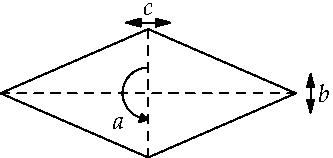
\includegraphics{group-rhombus}
			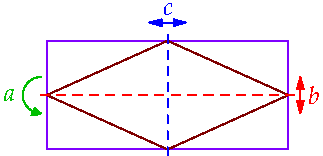
\includegraphics{group-klein}
		\end{minipage}
	\end{enumerate}
	  
% 	  \item The \emph{Klein four-group,\footnotemark} denoted $V$, is the symmetry group of a \textcolor{Purple}{rectangle} (or a \textcolor{Brown}{rhombus}): $e$ is the identity, $\textcolor{Green}{a}$ represents rotation by \ang{180}, and $\textcolor{red}{b},\textcolor{blue}{c}$ are reflections.
% 	\end{enumerate}
% 	\begin{center}
% 		\begin{minipage}[t]{0.25\linewidth}\vspace{-12pt}
% 		$\begin{array}[t]{c||c|c|c|c}
% 			\circ & e & \textcolor{Green}{a} & \textcolor{red}{b} & \textcolor{blue}{c}\\\hline\hline
% 			e & e & \textcolor{Green}{a} & \textcolor{red}{b} & \textcolor{blue}{c}\\\hline
% 			\textcolor{Green}{a} & \textcolor{Green}{a} & e & \textcolor{blue}{c} & \textcolor{red}{b}\\\hline
% 			\textcolor{red}{b} & \textcolor{red}{b} & \textcolor{blue}{c} & e & \textcolor{Green}{a}\\\hline
% 			\textcolor{blue}{c} & \textcolor{blue}{c} & \textcolor{red}{b} & \textcolor{Green}{a} & e
% 		\end{array}$
% 		\end{minipage}
% 		\begin{minipage}[t]{0.4\linewidth}\vspace{-17pt}
% 			\flushright
% 			%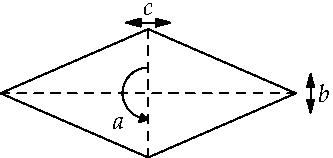
\includegraphics{group-rhombus}
% 			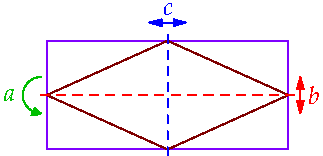
\includegraphics{group-klein}
% 		\end{minipage}
	%\end{center}
\end{defn}

\footnotetext{From the German \emph{Vierergruppe.} Felix Klein (1849--1925) was a pioneer in the application of group theory to geometry.}

Try drawing a smiley face on one side of a piece of paper and rotating/reflecting it until you believe Klein's example! 
	
\goodbreak

Since multiplication by an $n\times n$ matrix amounts to a function (e.g.\ $A\in \rM_n(\R)$ corresponds to a linear map $\R^n\to\R^n:\vx\mapsto A\vx$), we immediately conclude:

\begin{cor}{}{matrixmult}
	Multiplication of square matrices is associative.
\end{cor}

\begin{example}{}{gln}
	The \emph{general linear group} comprises the invertible $n\times n$ matrices under multiplication
	\[
		\rGL_n(\R)=\{A\in \rM_n(\R):\det A\neq 0\} \tag{non-abelian when $n\ge 2$}
	\]
	Invertibility is assumed, associativity is the corollary, and closure follows from the familiar result
	\[
		\det AB=\det A\det B
	\]
	Finally, the identity is multiplication by (drum roll\ldots) the \emph{identity matrix} $I=\smash{\scalebox{0.6}{%
	$\begin{pmatrix}
		1&0&&\\
		0&1&\ddots&\\
		&\ddots&\ddots&0\\
		&&0&1
	\end{pmatrix}$%
	}}$!!\smallbreak
	Does part 3 of Theorem \ref{thm:canc} now seem familiar?
\end{example}



\vfil

\begin{exercises}
	Key concepts/definitions/examples: make sure you can state the formal definitions
	\begin{quote}
		\emph{Group\,(closure,\,associativity,\,identity,\,inverse)\quad Commutativity/abelian\quad Cayley table}\par
		\emph{Rotation group $R_n$\quad Dihedral group $D_n$\quad Klein 4-group $V$\quad General linear group $\rGL_n(\R)$}
	\end{quote}


	\begin{enumerate}
	  \begin{minipage}[t]{0.72\linewidth}\vspace{-5pt}
			\item Given the binary operation table, calculate
			\begin{enumerate}\itemsep0pt
				\item \makebox[150pt][l]{$c\opast d$\hfill (b)\lstsp} $a\opast (c\opast b)$
				\item[(c)] \makebox[150pt][l]{$(c\opast b)\opast a$\hfill (d)\lstsp} $(d\opast c)\opast (b\opast a)$
			\end{enumerate}
		\end{minipage}
		\hfill
		\begin{minipage}[t]{0.2\linewidth}\vspace{-5pt}
			\flushright \scalebox{0.9}{%
				$\begin{array}{c||c|c|c|c}
					* & a & b & c & d\\\hline\hline
					a & c & d & a & b\\\hline
					b & d & c & b & a\\\hline
					c & a & b & c & d\\\hline
					d & b & a & d & c
				\end{array}$%
			}
		\end{minipage}
		\smallbreak
	
	
		\begin{minipage}[t]{0.72\linewidth}\vspace{0pt}
			\item A table for a binary operation on $\{a,b,c\}$ is given. Compute $a*(b*c)$ and $(a*b)*c$. Does the expression $a\opast b\opast c$ make sense? Explain why/why not.
			\end{minipage}
			\hfill
			\begin{minipage}[t]{0.2\linewidth}\vspace{0pt}
				\flushright\scalebox{0.9}{%
					$\begin{array}{c||c|c|c}
						* & a & b & c\\\hline\hline
						a & b & c & b\\\hline
						b & c & a & a\\\hline
						c & b & a & c
					\end{array}$%
				}
		\end{minipage}
		\par
	
	
		\item Are the binary operations in the previous questions commutative? Explain.
	
	
		\item\begin{enumerate}
		  \item Describe (\emph{don't write them all out!}) all possible binary operation tables on a set of two elements $\{a,b\}$. Of these, how many are commutative?
		  
		  \item How many commutative/non-commutative operations are there on a set of \emph{$n$} elements?\par
		  (\emph{Hint: a commutative table has what sort of symmetry?})
		\end{enumerate}
		
	  
	  \item Which are binary structures? For those that are, which are commutative and which associative?
	  \begin{enumerate}%
	    \item[(a)] \makebox[180pt]{$(\Z,*),\ a\opast b=a-b$\hfill (b)\lstsp} $(\R,*),\ a\opast b=2(a+b)$
	    
	    \item[(c)] \makebox[180pt]{$(\R,*),\ a\opast b=2a+b$\hfill (d)\lstsp} $(\R,*),\ a\opast b=\frac ab$\setcounter{enumii}{4}
	    
	    \item[(e)] \makebox[180pt]{$(\N,*),\ a\opast b=a^b$\hfill (f)\lstsp} $(\Q^+,*),\ a\opast  b=a^b$,  where $\Q^+=\{x\in\Q:x>0\}$
	    
	    \item[(g)] $(\N,*),\ a\opast b=$ product of the distinct prime factors of $ab$. Also define $1\opast 1=1$.\par
	    (e.g.~$42\opast 10=(2\cdot 3\cdot 7)\opast (2\cdot 5)=2\cdot 3\cdot 5\cdot 7=210$) 
	  \end{enumerate}
	  
	
	  \goodbreak
	  
	  
		\item For each axiom of an abelian group: if true, write it down; if false, provide a counter-example.
		\begin{enumerate}
		  \item \makebox[210pt]{$\N=\{1,2,3,\ldots\}$ under addition.\hfill (b)\lstsp} $\Q$ under multiplication.\setcounter{enumii}{2}
		  
		  \item[(c)] \makebox[210pt]{$X=\{a,b,c\}$ with $x\opast y:=y$.\hfill (d)\lstsp} $\R^3$ with the cross/vector product $\times$.\setcounter{enumii}{4}
		  
		  \item\label{exs:nzgroup} For each $n\in\R$, the set $n\Z=\{nz:z\in\Z\}$ of multiples of $n$ under addition.
	  \end{enumerate}
	  
	  
	  \item Determine whether each of the following sets of matrices is a group under multiplication.
	  \begin{enumerate}
	    \item \makebox[210pt]{$\mathcal K=\{A\in \rM_2(\R):\det A=\pm 1\}$\hfill (b)\lstsp} $\mathcal L=\{A\in \rM_2(\R):\det A=7\}$\setcounter{enumii}{2}
	    
	    \item $\mathcal N=\bigl\{\begin{smatrix}
	    a&b\\0&d
	    \end{smatrix}\in\rM_2(\R):ad\neq 0\bigr\}$
	  \end{enumerate}
	
	  
	  \item\begin{enumerate}
	    \item Prove the cancellation laws (Theorem \ref{thm:canc} parts 1 \& 2).
	    
	    \item True or false: in a group, if $xy=e$, then $y=x^{-1}$.
	    
	    \item\label{exs:multinverse2} In a (multiplicative) group, \emph{prove} that $(x^{-1})^n=(x^n)^{-1}$ for any $x$ and any $n\in\N$. How would we write this in an \emph{additive} group (see footnote \ref{fn:additive})?
	  \end{enumerate}
	    
	    
	  \item Let $G$ be a group. Prove the following:\vspace{-6pt}
	  \begin{enumerate}
	    \item $\forall x,y\in G,\ (xy x^{-1})^2=xy^2x^{-1}$
	    \qquad\qquad
	    (b) \ $\forall x\in G,\ (x^{-1})^{-1}=x$
	    \setcounter{enumii}{2}
	    
	    \item $G$ is abelian $\iff\forall x,y\in G,\ (xy)^{-1}=x^{-1}y^{-1}$
	  \end{enumerate}
	  
	  
	%   \item\label{exs:pullback} Prove or disprove: $(\R\setminus\{1\},*)$ is an abelian group, where $x\opast y=x+y-xy$.\par
	%   (\emph{Hint: factorize $x\opast y-1$})
	
	  
	  \item\begin{enumerate}%
		  \item\label{exs:funcnoncomm} Suppose $X$ contains at least two distinct elements $x\neq y$. Prove that there exist functions $f,g:X\to X$ for which $f\circ g\neq g\circ f$.
		  
			\item Show that multiplication of $n\times n$ matrices is non-commutative when $n\ge 2$.
		\end{enumerate}
	  
	  
	  \item\begin{enumerate}
	    \item Describe the symmetry group and Cayley table of a non-equilateral isosceles triangle.
	    
	    \item\label{exs:squarerot} Explicitly state the Cayley table for the rotation group $R_4$ of a square.
	    
	    \item Explain why the order of the dihedral group $D_n$ is $2n$.
	    
	    \item Prove the \emph{rotation} part of Corollary \ref{cor:rotationgroup}.
	  \end{enumerate}
		
		
	% 	\item The Lie bracket $[\ ,\ ]$ of two $n\times n$ matrices is defined by $[A,B]=AB-BA$.
	% 	\begin{enumerate}
	%   	\item Show that $[\ ,\ ]$ is an \emph{anti-commutative} binary operation on $\rM_n(\R)$, that is,
	% 		\[\forall A,B\in \rM_n(\R),\qquad [A,B]=-[B,A]\]
	% 		\item When $n=2$, give a counter-example to show that the Lie bracket is \emph{non-associative.}
	%   	\item Let $\fso(n)=\{A\in \rM_n(\R):A^T=-A\}$ be the set of skew-symmetric $n\times n$ matrices.
	% 		\begin{enumerate}
	%    		\item Is matrix multiplication a binary operation on $\fso(n)$?
	%    		\item Is the Lie bracket a binary operation on $\fso(n)$?
	% 		\end{enumerate}
	% 	\end{enumerate}
	  
	
	
	  \item Let $\mathcal U$ be a set and $\cP(\mathcal U)$ its power set (the set of subsets of $\mathcal U$).
	  \begin{enumerate}
	    \item Which of the group axioms is satisfied by the union operator $\cup$ on $\cP(\mathcal U)$?
	    
	    \item Repeat part (a) for the intersection operator.
	    
	    \item The \emph{symmetric difference} of sets $A,B\subseteq\mathcal U$ is the set
	    \[
	    	A\triangle B:=(A\cup B)\setminus(A\cap B)
	    \]
	    \begin{enumerate}
	      \item Use Venn diagrams to give a sketch argument that $\triangle$ is associative on $\cP(\mathcal U)$.
	      
	      \item Is $\bigl(\cP(\mathcal U),\triangle\bigr)$ a group? Explain your answer.
	  	\end{enumerate}
	  \end{enumerate}
	  
	  
	  \item\label{exs:magicsquare} (Magic Square)\quad Suppose $(G,*)$ is associative and $G$ is finite.\par
	  Prove that $(G,*)$ is a group if and only if its (multiplication) table satisfies two conditions:
			\begin{itemize}
			  \item[i.] One row and column (by convention the first) is a perfect copy of $G$ itself.
	  		\item[ii.] Every element of $G$ appears exactly once in each row and column.
			\end{itemize}
		
	 
	%   \item Let $C[0,1]$ denote the set of continuous functions $f:[0,1]\to\R$, and $C^1[0,1]$ the \emph{differentiable} functions for which $f'$ is continuous.
	% 	\begin{enumerate}
	% 		\item Define $*$ on $C^1[0,1]$ by
	% 		\[(f*g)(x):=\int_0^x f'(t)g'(t)\,\dt+f(0)+g(0)\]
	% 		Is $*$ a binary operation? Is it commutative? Associative? Prove your assertions.\par
	% 		(\emph{Hint: use the Fundamental Theorem of Calculus})
	% 		
	%     \item Suppose $e\in C^1[0,1]$ is an identity for $*$. Show that $e$ satisfies the integral equation
	%     \[\int_0^x f'(t)e'(t)\,\dt+f(0)+e(0)=f(x)\]
	%     for all functions $f\in C^1[0,1]$. Does such an $e$ exist? Is it unique?
	%     
	%     \item (If you've done a little analysis)\quad Define $*$ by
	%     \[f*g=\begin{cases} f\ \mathrm{if}\ \max f\ge \max g,\\ g\ \mathrm{if}\ \max g > \max f. \end{cases}\]
	%     Which result from elementary analysis guarantees that this is a binary operation on $C[0,1]$? Is the binary operation commutative? Does it have an identity? Explain your answer.
	%   \end{enumerate}
	  
	\end{enumerate}
\end{exercises}

\clearpage



\subsection{Subgroups}\label{sec:subgroup}

The prefix \emph{sub-} in mathematics usually indicates a \emph{subset} that retains whatever structure follows.

\begin{defn}{Subgroup}{}
	Let $G$ be a group. A \emph{subgroup} of $G$ is a subset $H\subseteq G$ which remains a group with respect to the \emph{same} binary operation. We write $H\le G$.\smallbreak
	A subgroup $H$ is a \emph{proper subgroup} if $H\neq G$. This is written $H<G$.\smallbreak
	The \emph{trivial subgroup} is the 1-element set $\{e\}$; all other subgroups are \emph{non-trivial}.
\end{defn}


\begin{examples}{}{basicsubgroup}
	The following should be immediate from the definition.
	\begin{enumerate}\itemsep2pt
	  \item\label{ex:basicsubgroup1} \makebox[230pt]{$\{e\}\le G$ and $G\le G$ for \emph{any} $G$ \hfill 2.\lstsp}$(\Z,+)<(\Q,+)<(\R,+)<(\C,+)$
		\item[3.] \makebox[230pt]{$(\Q^\times,\cdot)<(\R^\times,\cdot)<(\C^\times,\cdot)$ \hfill 4.\lstsp}$(\R^n,+)<(\C^n,+)$
	% 	\item $(\R^m,+)\le (\R^n,+)$ if $m\le n$. This can be visualized in many ways, the simplest is to consider $\R^m=\Span\{\vect em\}\le \R^n=\Span\{\vect en\}$: the subgroup consists of all column vectors whose last $n-m$ entries are zero.
		\item[5.] \makebox[230pt]{$(2\Z,+)<(\Z,+)$  \hfill 6.\lstsp} $(R_3,\circ)\le (R_6,\circ)$\quad (rotation groups)
		%\item $(C(\R),+)<(C^1(\R),+)$ (all differentiable functions are continuous)
	\end{enumerate}
\end{examples}

Thankfully one doesn't have to check all the group axioms to see that a subset is a subgroup.

\begin{thm}{Subgroup criterion}{subgroup}
	Let $G$ be a group. A non-empty subset $H\subseteq G$ is a subgroup if and only if it is closed under the group operation and inverses. Otherwise said,
	\[
		\forall h,k\in H,\ hk\in H \text{ and }  h^{-1}\in H
	\]
\end{thm}

\begin{proof}
	($\Rightarrow$) \ $H$ is a group and therefore satisfies all the axioms, including closure and inverse.\smallbreak
	$(\Leftarrow$) \ Since $H$ is a subset of $G$, the group operation on $G$ is automatically associative\footnotemark{} on $H$. By assumption, $H$ also satisfies the closure and inverse axioms, so it remains only to check the identity.\smallbreak
	Since $H\neq\emptyset$, we may choose some (any!) $h\in H$, from which
	\[
		e=hh^{-1}\in H
	\]
	since inverses and products remain in $H$. The identity $e$ of $G$ therefore in $H$, and so $H$ is a group.
\end{proof}

\footnotetext{Definition \ref{defn:assoc} makes no claim as to \emph{where} $x(yz)=(xy)z$ lives!}

\vspace{-5pt}

\begin{examples}{}{}
	\exstart All of Examples \ref{ex:basicsubgroup} can be confirmed using the theorem. For instance,
	\[
		2\Z=\{\ldots,-2,0,2,4,\ldots\}=\{2z:z\in\Z\}
	\]
	is certainly a non-empty subset of the integers. Moreover, if $2m,2n\in 2\Z$, then
	\[
		2m+2n=2(m+n)\in 2\Z\quad \text{and}\quad \!-(2m)=2(-m)\in 2\Z
	\]
	whence $2\Z$ is closed under addition and inverses (negation).
	\begin{enumerate}\setcounter{enumi}{1}
	  \item The positive integers $\N=\{1,2,\ldots \}$ are closed under addition but not inverses (for instance no $x\in\N$ satisfies $x+2=0$). Thus $\N$ is not a subgroup of $\Z$ under addition.
		\item\label{intro:modex} Let $1+3\Z$ be the set of integers with remainder 1 when divided by 3:
		\[
			1+3\Z=\{1+3n:n\in\Z\}=\{1,4,7,10,13,\ldots, -2,-5,-8,\ldots\}
		\]
		Since $1\in 1+3\Z$ but $1+1=2\not\in 1+3\Z$, we see that $1+3\Z$ is not a subgroup of $(\Z,+)$.
	\end{enumerate}
\end{examples}


\goodbreak


\begin{minipage}[t]{0.83\linewidth}\vspace{0pt}
	\boldinline{Subgroup Diagrams}
	
	It can be helpful to represent subgroup relations pictorially, where a descending line indicates a subgroup relationship. For instance, the diagram on the right summarizes \emph{four} subgroup relations
	\[
		6\Z<2\Z<\Z\quad\text{and}\quad 6\Z<3\Z<\Z
	\]
\end{minipage}
\hfill
\begin{minipage}[t]{0.15\linewidth}\vspace{0pt}
	\flushright$\xymatrix @C5pt @R12pt{%
		& \Z \ar@{-}[dl] \ar@{-}[dr] &\\
		2\Z \ar@{-}[dr] & & 3\Z \ar@{-}[dl]\\
		& 6\Z &\\
	}$
\end{minipage}
\medbreak
where all four are groups under addition. If $G$ has only \emph{finitely many subgroups,} then its \emph{subgroup diagram} is the complete depiction of all subgroups.


\boldinline{Matrix subgroups}

In Example \ref{ex:gln} we saw that the invertible matrices $\rGL_n(\R)$ form a group under multiplication. Here is one of its many subgroups, some others are in Exercise \ref{exs:subgpmatrix}.

\begin{example}{}{orthogonal}
The set $\rO_n(\R)=\{A\in\rM_n(\R):A^TA=I\}$ forms a subgroup of $\rGL_n(\R)$.
	\begin{itemize}\itemsep0pt
	  \item $I\in \rO_n(\R)$ so we have a non-empty set. Moreover, if $A\in \rO_n(\R)$, then
	  \[
	  	1=\det I=\det A\det A^T=(\det A)^2\implies \det A\neq 0\implies A\in\rGL_n(\R)
	  \]
	  \item If $A,B\in\rO_n(\R)$, then
	  \begin{gather*}
	  	(AB)^T(AB)=B^TA^TAB=B^TIB=B^TB=I,\quad\text{and,}\\
	  	(A^{-1})^TA^{-1}=(A^T)^TA^T=(AA^T)^T=I^T=I
	  \end{gather*}
	  whence $AB$ and $A^{-1}\in\rO_n(\R)$.
	\end{itemize}
	We call this the \emph{orthogonal group.} When $n=2$ or 3, its elements may be recognized as rotations and reflections. For instance, the matrix $\frac 1{\sqrt 2}
	\begin{smatrix}
		1&-1\\
		1&1
	\end{smatrix}
	\in\rO_2(\R)$ rotates $\R^2$ counter-clockwise by \ang{45}.
\end{example}



\boldinline{Geometric subgroup proofs}\hypertarget{sec:geomdih}{}

Arranging figures such that every symmetry of one is also a symmetry of the other immediately results in a subgroup relationship!

% \begin{example}[lower separated=false, sidebyside, sidebyside align=top seam, sidebyside gap=0pt, righthand width=0.33\linewidth]{}{}
% The Klein four-group was \emph{defined} geometrically! Since each non-identity element $a,b,c$ is its own inverse, we have \emph{three distinct} proper non-trivial subgroups, each containing two elements,
% \[\{e,a\},\quad\{e,b\},\quad\{e,c\}\]
% Why are there no other interesting subgroups? If $a$ and $b$ both lie in a subgroup, then so must $ab=c$ and we'd obtain the entirety of $V$! The same argument applies to the other pairs.
% \tcblower
%  \flushright$\xymatrix{ & V \ar@{-}[dl] \ar@{-}[dr] \ar@{-}[d] & \\
%  \{e,a\} & \{e,b\} & \{e,c\} \\
%  & \{e\} \ar@{-}[ul] \ar@{-}[ur] \ar@{-}[u] &
% }$
% \end{example}



\begin{example}[lower separated=false, sidebyside, sidebyside align=top seam, sidebyside gap=0pt, righthand width=0.33\linewidth]{}{hexsubgroup}
	A \textcolor{blue}{regular hexagon} has symmetry group $D_6=\{\rho_0,\ldots,\rho_5,\mu_0,\ldots,\mu_5\}$ consisting of six rotations and six reflections:
	\begin{itemize}
	  \item $\rho_k$ is rotation counter-clockwise by $\ang{60k}$; the identity is $\rho_0$.
	  \item The $\mu_k$ are reflections across `diameters' of the hexagon as indicated in the pictures below.
	\end{itemize}
	
	Now draw two \textcolor{red}{equilateral triangles} inside the hexagon.	Each of the six symmetries of the equilateral triangle is also a symmetry of the hexagon! Since both are groups under the same operation (composition of functions), it follows that the symmetry group $D_3$ of the triangle is a subgroup of $D_6$, indeed in two different ways:
	\[
		\{e,\rho_2,\rho_4,\mu_0,\mu_2,\mu_4\}< D_6\quad\text{and}\quad \{e,\rho_2,\rho_4,\mu_1,\mu_3,\mu_5\}< D_6
	\]
	\tcblower
	\flushright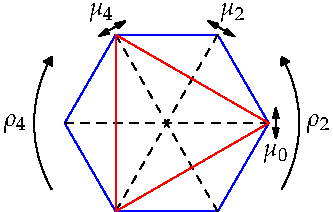
\includegraphics[scale=0.9]{group-hexagon1}\\
	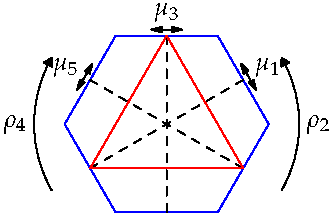
\includegraphics[scale=0.9]{group-hexagon2}
\end{example}

The key takeaway here is that subgroup relations are \emph{everywhere} in mathematics.

% We'll properly discuss the groups in this example in Chapter \ref{chap:perm}.

\goodbreak

\begin{exercises}
	Key concepts/definitions:\quad \emph{(Proper/trivial/non-trivial) Subgroup}
	\begin{quote}
		\emph{Closure under operation/inverses\quad Subgroup diagram}
	\end{quote}
	
	
	\begin{enumerate}
	  \item Use Theorem \ref{thm:subgroup} to verify that $\Q^\times$ is a subgroup of $\R^\times$ under multiplication.
	  
	  
		\item Give two reasons why the \emph{non-zero} integers do not form a subgroup of $\Z$ under addition.
	  	
	  	
	  \item Describe/explain the relationship between positive integers $m$ and $n$ if $(m\Z,+)\le (n\Z,+)$.
	
	
	  \item Prove or disprove: the set $H=\{\frac a{2^n}:a\in\Z,n\in\N_0\}$ forms a group under addition.
	    
	    
	  \item Use Theorem \ref{thm:subgroup} to explain why the set of \emph{rotations} of a planar geometric figure is a subgroup of the group of its rotations \emph{and} reflections.
	  
	 
	  \item\begin{enumerate}
	    \item Find the complete subgroup diagram of the Klein four-group.
	    
	  	\item Modelling Example \ref{ex:hexsubgroup}, draw three pictures which describe different ways in which the Klein four-group may be viewed as a subgroup of $D_6$.
	  \end{enumerate}
	  
	  
	  \item Find the subgroups and subgroup diagram of the rotation group $R_6=\{\rho_0,\ldots,\rho_5\}$, where $\rho_k$ is counter-clockwise rotation by $\ang{60k}$. 
	  
	  
	%   \item\begin{enumerate}
	%     \item How many elements are in the rotation group of a regular tetrahedron?\par
	%     (\emph{Hint: any face can be rotated to any other and then oriented\ldots})
	%     \item Repeat the question for a cube and a regular octahedron. Your answer should be the \emph{same}: can you think of a \emph{geometric} reason why?\par
	%     (\emph{Hint: what does an octahedron have six of?})
	% %     \item How large are the rotation groups of the tetrahedron, dodecahedron and icosahedron?There are three other platonic solids. What about the dodecahedron and the icosahedron?
	%   \end{enumerate}
	  
	  
		\item Suppose $H$ and $K$ are subgroups of $G$. Prove that $H\cap K$ is also a subgroup of $G$.
	   
	   
		\item Let $H$ be a non-empty subset of a group $G$. Prove that $H$ is a subgroup of $G$ if and only if
	  \[
	  	\forall x,y\in H,\ xy^{-1}\in H
	  \]
	  
	  
	  \item\label{exs:subgpmatrix} Prove that each set of matrices forms a group under multiplication (unless you love matrices, don't feel you have to memorize these).
	  \begin{enumerate}
	    \item Special linear group: $\rSL_n(\R)=\bigl\{A\in \rM_n(\R):\det A=1\bigr\}$
	    
	    \item Special orthogonal group: $\rSO_n(\R)=\{A\in\rM_n(\R):A^TA=I\text{ and }\det A=1\}$
	    
	    \item $\mathcal Q_n=\bigl\{A\in \rM_n(\R):\det A\in\Q^\times\bigr\}$
	    
	    \item (Harder)\lstsp Symplectic group: $\rSp_{2n}(\R)=\bigl\{A\in \rM_{2n}(\R):A^TJA=J\bigr\}$, where $J=\scalebox{0.6}{$\left(\!
	    \begin{array}{c|c}
	    	0&I_n\\
	    	\hline -I_n&0
	    \end{array}
	    \!\right)$}$ is a block matrix and $I_n$ the $n\times n$ identity matrix.
	    
	    \item (Hard)\lstsp $\rSL_n(\Z)=\bigl\{A\in \rM_n(\Z):\det A=1\bigr\}$: all entries in these matrices are \emph{integers.}\par
	    (\emph{Hint: look up the classical adjoint $\operatorname{adj}A$ of a square matrix})
	  \end{enumerate}
	  Now construct a diagram showing the subgroup relationships between the groups
	  \[
	  	\rGL_n(\R),\quad \rSL_n(\R),\quad \rO_n(\R),\quad \rSO_n(\R),\quad \mathcal Q_n,\quad \rSL_n(\Z)\tag{\emph{ignore $\rSp_{2n}(\R)$}}
	  \]
	  
	 	
	 	\item\label{exs:quaternion} (Hard)\lstsp $Q_8=\{\pm 1,\pm i,\pm j,\pm k\}$ forms a group under `multiplication' subject to the properties:
	  \begin{itemize}\itemsep0pt
	    \item 1 is the identity.
	    \item $-1$ commutes with everything; e.g.\ $(-1)i=-i=i(-1)$, etc.
	    \item $(-1)^2=1$,\quad $i^2=j^2=k^2=-1$ \ and \ $ij=k$.
	    \item Multiplication is associative.
	  \end{itemize}
	  \begin{enumerate}
	    \item Find the Cayley table of $(Q_8,\cdot)$.\par
	  	(\emph{Hint: You should easily be able to fill in 44 of 64 entries; now use associativity\ldots})
	  
	  	\item Find all subgroups of $Q_8$ and draw its subgroup diagram.
		\end{enumerate}
	 
	\end{enumerate}
\end{exercises}


\clearpage



\subsection{Homomorphisms \& Isomorphisms}\label{sec:morph}

A key goal of abstract mathematics is the comparison of similar/identical structures with outwardly different appearances. Our method of comparison is to use \emph{functions.}

\begin{defn}{Homomorphism}{homo}
	Suppose $(G,\ast)$ and $(H,\star)$ are binary structures and $\phi:G\to H$ a function. We say that $\phi$ is a \emph{homomorphism} of binary structures if
	\[
		\forall x,y\in G,\ \phi(x\opast y)=\phi(x)\opstar\phi(y)
	\]
\end{defn}

For most of these notes (certainly after this chapter), all binary structures will be groups.



\begin{examples}{}{}
	\exstart The%
	\def\opbl{\mathbin{\textcolor{blue}{+}}}
	\def\oprd{\mathbin{\textcolor{red}{+}}} 
	function $\phi:(\N,\textcolor{red}{+})\to(\R,\textcolor{blue}{+})$ defined by $\phi(x)=\sqrt 2x$ is a homomorphism,\vspace{-2pt}
	\[
		\phi(x\oprd y)=\sqrt 2(x\oprd y)=\sqrt 2x\opbl \sqrt 2y=\phi(x)\opbl \phi(y)
	\]
	It is worth spelling this out since there are \emph{two} ways to combine addition and $\phi$:\vspace{-5pt}
	\begin{enumerate}\setcounter{enumi}{1}\itemsep2pt
	  \item[]\begin{itemize}
	  	\item Sum $x\oprd y$, then map to $\R$ to obtain $\phi(x\oprd y)$.
	  	\item Map to $\R$, then sum to obtain $\phi(x)\opbl\phi(y)$.
		\end{itemize}
		The homomorphism property says the results are \emph{always identical.}
		
	  \item If $V,W$ are vector spaces then every linear map $\rT:V\to W$ is a group homomorphism:\footnotemark
	  \[
	  	\forall\vv_1,\vv_2\in V,\quad \rT(\vv_1+\vv_2)=\rT(\vv_1)+\rT(\vv_2)
	  \]
	  You've been encountering homomorphisms your entire mathematical career, even in calculus: $\diff x(f+g)=\diff[f]{x}+\diff[g]{x}$ is a homomorphism property! 
	\end{enumerate}
\end{examples}


\footnotetext{The scalar multiplication condition $\rT(\lambda\vv)=\lambda \rT(\vv)$ of a linear map is not relevant here.}

The most useful homomorphisms are \emph{bijective}, so much so that they get a special name.

\begin{defn}{Isomorphism}{iso}
	An \emph{isomorphism} is a bijective/invertible homomorphism.\footnotemark\par
	We say that $G$ and $H$ are \emph{isomorphic,} written $G\cong H$, if there exists an isomorphism $\phi:G\to H$.
\end{defn}

\footnotetext{These terms come from ancient Greek: \emph{homo-} (similar, alike), \emph{iso-} (equal, identical), and \emph{morph(e)} (shape, structure).}

Why do we care about isomorphisms? Because \emph{isomorphic structures are essentially identical}: one is simply a relabelled version of the other!\medbreak


Here is the standard procedure for showing that binary structures $(G,*)$ and $(H,\star)$ are isomorphic:
\begin{enumerate}\itemsep2pt
	\item (\emph{Definition})\lstsp Define $\phi:G\to H$, if necessary.\footnote{As we'll see later (e.g., Theorem \ref{thm:cyclicisomorph}), if $G$ is a set of equivalence classes you might need to check that $\phi$ is \emph{well-defined.}}
	\item (\emph{Homomorphism})\lstsp Verify that $\phi(x\opast y)=\phi(x)\opstar\phi(y)$ for all $x,y\in G$.
	\item (\emph{Injectivity/1--1})\lstsp Check $\phi(x)=\phi(y)\implies x=y$.
	\item (\emph{Surjectivity/onto})\lstsp Check $\operatorname{range}\phi=H$. Equivalently $\forall h\in H,\ \exists g\in G$ such that $h=\phi(g)$.
\end{enumerate}

The last three steps can be done in any order. Injectivity/surjectivity can be combined if you exhibit an explicit \emph{inverse function} $\phi^{-1}:H\to G$.


\goodbreak


\begin{examples}{}{expiso}
	\exstart We show that $(2\Z,+)$ and $(3\Z,+)$ are isomorphic groups.\vspace{-2pt}
	\begin{enumerate}\setcounter{enumi}{1}
	  \item[]\begin{description}
	  	\item[\normalfont\emph{Definition}:] The obvious function is $\phi(x)=\frac 32x$. Plainly $\phi(2m)=3n$ whence $\phi:2\Z\to 3\Z$.
	  	\item[\normalfont\emph{Homomorphism}:] $\phi(x+y)=\frac 32(x+y)=\frac 32x+\frac 32y=\phi(x)+\phi(y)$
	  	\item[\normalfont\emph{Injectivity}:] $\phi(x)=\phi(y)\implies \frac 32x=\frac 32y\implies x=y$.
	  	\item[\normalfont\emph{Surjectivity}:] If $z=3n\in 3\Z$, then $z=\frac 32\cdot\frac 23z=\frac 32(2n)=\phi(2n)\in\operatorname{range}\phi$.
		\end{description}
		The last step is essentially the observation that $\phi^{-1}(z)=\frac 23z$.\smallbreak
		More generally, the groups $(m\Z,+)$ and $(n\Z,+)$ are isomorphic whenever $m,n\neq 0$. 
	
		\item\label{ex:expiso1}	The function $\phi(x)=e^x$ is an isomorphism of abelian groups $\phi:(\R,+)\cong(\R^+,\cdot)$.\vspace{-2pt}
		\begin{description}%\itemsep2pt
	  	\item[\normalfont\emph{Definition}:] This is unnecessary since $\phi$ is given. However, note that both domain and codomain are \emph{abelian groups} and that $\R^+=(0,\infty)$ means the \emph{positive real numbers.}
	  	\item[\normalfont\emph{Homomorphism}:] This is the familiar exponential law (group theory is everywhere!)
	  	\[
	  		\phi(x+y)=e^{x+y}=e^xe^y=\phi(x)\phi(y)
	  	\]
	  	\item[\normalfont\emph{Bijectivity}:] $\phi^{-1}(z)=\ln z$ is the inverse function of $\phi$.
		\end{description}
	\end{enumerate}
\end{examples}



\boldinline{Non-isomorphicity \& Structural Properties}

Unless sets are very small, it is unrealistic to test every function $\phi:G\to H$ to see that structures are non-isomorphic! Instead we have to be a little more cunning.

	
\begin{defn}{Structural properties}{}
	A \emph{structural property} is any property which is preserved under isomorphism: if $\phi:(G,*)\to (H,\star)$ is an isomorphism then $(G,*)$ and $(H,\star)$ have identical structural properties.
\end{defn}


Suppose $\phi:(G,*)\to (H,\star)$ is an isomorphism. Here is a non-exhaustive list of structural properties; we'll check some in Exercise \ref{exs:structural1}.
\begin{description}
  \item[\normalfont\emph{Cardinality/order}:] Since $G$ and $H$ are bijectively paired, their cardinalities are the same.
  \item[\normalfont\emph{Commutativity \& Associativity}:] For instance, if $\ast$ is commutative, then
  \[
  	\forall x,y\in G,\ \phi(x)\opstar\phi(y)=\phi(x\opast y)=\phi(y\opast x)=\phi(y)\opstar\phi(x)
  \]
  Since $\phi$ is bijective, this says that $\star$ is commutative on $H$.
  \item[\normalfont\emph{Identities \& Inverses}:] If $G$ has identity $e$, then $\phi(e)$ is the identity for $H$. Similarly $\phi$ maps inverses to inverses.
  \item[\normalfont\emph{Solutions to equations}:] Related equations in $G$ and $H$ have the same number of solutions: e.g.
  \[x\opast x=x\iff \phi(x)\opstar\phi(x)=\phi(x)\]
  The equations $x\opast x=x$ and $z\opstar z=z$ therefore have the same number of solutions.%\footnotemark
  \item[\normalfont\emph{Being a group}] If $G$ is a group, so also is $H$.
\end{description}

%\footnotetext{Such solutions are called \emph{idempotents}; thus existence of idempotents is a structural property.}

\goodbreak

\begin{examples}{}{}
	\exstart Since $\N_0=\{0,1,2,3,\ldots\}$ contains an identity element 0 while $\N$ does not, we conclude that the binary structures $(\N_0,+)$ and $(\N,+)$ are non-isomorphic..

	\begin{enumerate}\setcounter{enumi}{1}\itemsep2pt
	  \begin{minipage}[t]{0.72\linewidth}\vspace{-5pt}
	  	\item The binary structures defined by the two tables are non-isomorphic; the first is commutative while the second is not.
	  \end{minipage}
	  \hfill
	  \begin{minipage}[t]{0.27\linewidth}\vspace{-5pt}
		  \flushright%
		  $\begin{array}[t]{c||c|c}
				* & a & b\\
				\hline\hline a & a & b\\
				\hline b & b & a
		  \end{array}
		  \quad
		  \begin{array}[t]{c||c|c}
				\star & c & d\\
				\hline\hline c & c & d\\
				\hline d & c & d
		  \end{array}$
	  \end{minipage}
	  \par 
	% 	
	%   \item The groups $(\Z_6,+_6)$ and $D_3$ both have order six, but are non-isomorphic since $\Z_6$ is abelian and $D_3$ is not.
	  
	  \item To see that $(\Q,+)$ and $(\R,+)$ are non-isomorphic groups, it is enough to recall that the sets have different cardinalities: $\Q$ is \emph{countably infinite} while $\R$ is \emph{uncountable.}
	  
	  \item $\rGL_2(\R)$ and $(\R,+)$ have the same cardinality. However, since the first is non-abelian and the second abelian, the two groups are non-isomorphic. 
	\end{enumerate}
\end{examples}

Many properties are non-structural and therefore \emph{cannot} be used to show non-isomorphicity: the type of element (number, matrix, etc.), the type of binary operation (addition, multiplication, etc.).



\boldinline{Transferring a Binary Structure}


We can convert a bijection into an isomorphism simply by imposing the homomorphism property. If $(H,\star)$ and a bijection $\phi:G\to H$ are given, we can \emph{define} a binary operation $\ast$ on $G$ by \emph{pulling-back} $\star$:
\[
	\forall x,y\in G,\ x\opast y:=\phi^{-1}\bigl(\phi(x)\opstar\phi(y)\bigr)
\]
Plainly $\phi:(G,*)\cong(H,\star)$ is an isomorphism! We can similarly \emph{push-forward} a binary  structure from $G$ to $H$ using a bijection:
\[
	w\opstar z:=\phi\bigl(\phi^{-1}(w)\opast\phi^{-1}(z)\bigr)
\]

\begin{example}{}{pull-back}
% \exstart As already seen, $\phi:2\Z\to3\Z:x\mapsto\frac 32x$ is a bijection. Define $\star$ on $3\Z$ by
% \[w\opstar z:=\frac 13wz \tag{$3m\opstar 3n=\frac 13(3m)(3n)=3mn\in 3\Z$}\]
% The pull-back of $\star$ to $2\Z$ is then
% \[x\opast y= \frac 23\left(\frac 32 x\opstar\frac 32y \right) =\frac 23\cdot \frac 34xy=\frac 12xy\]
% which is easily confirmed to be a binary operation on $2\Z$. Since $\phi$ is an isomorphism, we can verify certain shared structural properties:
% \begin{quote}
% \begin{description}
%   \item[\normalfont\emph{Cardinality}:] $2\Z$ and $3\Z$ are both uncountably infinite sets.
%   \item[\normalfont\emph{Commutativity \& Associativity}:] Both are commutative and associative, e.g.
%   \[a\opast (b\opast c)=(a\opast b)\opast c=\frac 14abc\]
%   \item[\normalfont\emph{Identities}:] $(2\Z,\ast)$ has identity 2 (e.g.\ $2\opast x=\frac 12\cdot 2x=x$) and $(3\Z,\star)$ has identity $\phi(2)=3$.
%   \item[\normalfont\emph{Inverses}:] Neither has inverses and therefore neither is a group: e.g. $4\in 2\Z$ has no inverse
%   \[4\opast x=2\iff 2x=2\iff x=1\not\in 2\Z\]
% \end{description}
% \end{quote}
%\begin{enumerate}\setcounter{enumi}{1}
  %\item 
  The function $\phi(x)=x^3+8$ is a bijection $\R\to\R$. If $\phi:(\R,*)\to(\R,+)$ is an isomorphism, then the operation $\ast$ must be
	\[
		x\opast y:=\phi^{-1}\bigl(\phi(x)+\phi(y)\bigr) =\phi^{-1}(x^3+y^3+16) =\sqrt[3]{x^3+y^3+8}
	\]
	Since $(\R,+)$ is an abelian group and $\phi^{-1}$ an isomorphism, $(\R,*)$ must also be an abelian group. Moreover, its identity must be
	\[
		\phi^{-1}(0)=\sqrt[3]{-8}=-2
	\]
	As a sanity check, observe that
	\[
		x\opast (-2)=\sqrt[3]{x^3+(-2)^3+8}=x
	\]
%\end{enumerate}
\end{example}


\bigskip


\begin{minipage}[t]{0.85\linewidth}\vspace{-10pt}
	\boldinline{Up to Isomorphism: a common shorthand}\phantomsection\label{sec:uptoiso} This phrase is ubiquitous in abstract mathematics. For an example of how it is used, recall that if $(\{e,a\},*)$ is a group with identity $e$, then its Cayley table must be as shown (Example \ref*{ex:rx}.\ref{ex:smallcayley1}). Said formally:
\end{minipage}
\hfill
\begin{minipage}[t]{0.14\linewidth}\vspace{-10pt}
	\flushright%
	$\begin{array}[t]{c||c|c}
		* & e & a\\\hline\hline
		e & e & a\\\hline
		a & a & e
	\end{array}$
\end{minipage}\par

\begin{quote}
	\emph{Up to isomorphism,} there exists a unique group of order two.
\end{quote}

More precisely: if $G$ is \emph{any} group of order two, then there exists an isomorphism $\phi:\{e,a\}\to G$. The expression `up to isomorphism' is essential, for without it the sentence is \emph{false}: there are \emph{infinitely many distinct groups of order two, but all are isomorphic.}

\goodbreak


With its focus on functions rather than sets and its long list of unfamiliar words, this last introductory section likely seems the hardest of the three. Complete fluency with the vocabulary is \emph{not required} at this stage. The next few chapters will focus on several standard families of groups, providing plenty opportunity to reinforce the language introduced in this chapter.

\begin{exercises}{}
	Key concepts/definitions:\quad \emph{Homomorphism\quad Injective/surjective/bijective}
	\begin{quote}
		\emph{Isomorphism\quad Structural property\quad `Up to isomorphism'}
	\end{quote}
	
	\begin{enumerate}
		\item Which of the following are homomorphisms/isomorphisms of binary structures? Explain.
	  \begin{enumerate}
	    \item \makebox[210pt][l]{$\phi:(\Z,+)\to (\Z,+)$, \ $\phi(n)=-n$\hfill (b)\lstsp} $\phi:(\Z,+)\to (\Z,+)$, \ $\phi(n)=n+1$
	    
	    \item[(c)] \makebox[210pt][l]{$\phi:(\Q,+)\to (\Q,+)$, \ $\phi(x)=\frac{4}{3}x$\hfill (d)\lstsp} $\phi:(\Q,\cdot)\to (\Q,\cdot)$, \ $\phi(x)=x^2$
	    
	    \item[(e)] \makebox[210pt][l]{$\phi:(\R,\cdot)\to (\R,\cdot)$, \ $\phi(x)=x^5$\hfill (f)\lstsp} $\phi:(\R,+)\to (\R,\cdot)$, \ $\phi(x)=2^x$
	    
	    \item[(g)] $\phi:(\rM_2(\R),\cdot)\to (\R,\cdot)$, \ $\phi(A)=\det A$
	    
	    \item[(h)] $\phi:(\rM_n(\R),+)\to (\R,+)$, $\phi(A)=\tr A=$ trace of the matrix $A$ (add the entries on the main diagonal).
	  \end{enumerate}
	  
	  
	  \item Show that $(\Z,+)\cong (n\Z,+)$ for any \emph{non-zero} constant $n$.
	  
	  
	  \item Prove or disprove: $(\R^3,+)\cong(\R^3,\times)$ (cross product). 
	  
	  
	  \item $\phi(n)=2-n$ is a bijection of $\Z$ with itself. For each of the following, define a binary relation $*$ on $\Z$ such that $\phi$ is an isomorphism of binary relations.
	  \begin{enumerate}
	    \item $\phi:(\Z,*)\cong (\Z,+)$\quad\qquad
	    (b) \ $\phi:(\Z,*)\cong (\Z,\cdot)$\quad\qquad 
	    (c) \ $\phi:(\Z,*)\cong (\Z,\max(a,b))$
	  \end{enumerate}
	  (\emph{Hint: read Example \ref{ex:pull-back}})
	  
	  
		\item $\phi(x)=x^2$ is a bijection $\phi:\R^+\to\R^+$. Find $x\opast y$ if $\phi$ is to be an isomorphism of binary structures
		\begin{enumerate}
		  \item $\phi:(\R^+,\ast)\to(\R^+,+)$ \qquad\qquad (b) \ $\phi:(\R^+,+)\to(\R^+,\ast)$
		\end{enumerate}
	  
	  
	%   \item Recall Show that $x\opast y=x+y-xy$ is the pull-back of $(\R^\times,\cdot)$ by $\phi(x)=1-x$. Hence provide a much faster argument that $(\R\setminus\{1\},*)$ is an abelian group.
	
	  
	  \item\label{exs:structural1} Suppose $\phi:(G,*)\to (H,\star)$ is an isomorphism of binary structures. Prove the following:
	  \begin{enumerate}
	    \item\label{exs:structidentity} If $e$ is an identity for $G$, then $\phi(e)$ is an identity for $H$.
	    
	    \item If $x\in G$ has an inverse $y$, then $\phi(x)\in H$ has an inverse $\phi(y)$.
	    
	    \item If $*$ is associative, so is $\star$.
	  \end{enumerate}
	  
	  
	  \item Let $\phi:(G,*)\to (H,\star)$ be a homomorphism of binary structures. Prove that the \emph{image}
	  \[
	  	\phi(G)=\image \phi=\{\phi(x):x\in G\}
	  \]
	  is closed under $\star$ (thus $(\phi(G),\star)$ is a binary structure). If $(G,*)$ and $(H,\star)$ are both groups, show that $\phi(G)$ is a subgroup of $H$.
	  
	  
	  \item Revisit Exercise \ref{exs:structidentity}. Suppose $e$ is an identity for $(G,*)$ and that $\phi:G\to H$ is merely a \emph{homomorphism.} Must $\phi(e)$ be an identity for $H$? Explain why/why not. Does it matter whether $\phi$ is a homomorphism of \emph{groups}?
	  
	  
	  \item Let $G$ be the group of rotations of the plane about the origin under composition.
	  \begin{enumerate}
			\item Show that $\phi:(\R,+)\to G$ defined by
			\[
				\phi(x)=\text{rotate counter-clockwise $x$ radians}
			\]
	  	is a homomorphism of groups.
	  	
			\item Prove or disprove: $\phi$ is an \emph{isomorphism.}
		\end{enumerate}
		
	
	  \item\begin{enumerate}
	    \item Prove that $S:=\left\{
	    \begin{smatrix}
	    	a&-b\\
	    	b&a
	    \end{smatrix}
	    \in \rM_2(\R)\right\}$ forms a group under matrix addition.
	    
	    \item Prove that $T=S\setminus\{0\}$ \ ($S$ without the zero matrix) forms a group under matrix \emph{multiplication.}
	    \item Define $\phi
	    \begin{smatrix}
		    a&-b\\
		    b&a
	    \end{smatrix}
	    =a+ib$. Prove that $\phi:S\to\C$ and $\phi_T:T\to\C^\times$ are \emph{both} isomorphisms
	    \[
	    	\phi:(S,+)\cong(\C,+),\qquad \at\phi T:(T,\cdot)\cong(\C^\times,\cdot)
	    \]
	    (\emph{In a future class, $\phi$ will be described as an isomorphism of rings/fields})
	  \end{enumerate}
	  
	  
	% 	\item A group structure on $X=(-\frac\pi 2,\frac\pi 2)$ could be defined as follows:
	% 	\[\forall x_1,x_2\in X,\text{ define }x_1*x_2=\tan^{-1}(\tan(x)+\tan(y))\]
	% 	Since $\tan:(-\frac\pi 2,\frac\pi 2)\to\R$ is a bijection, we see that $*$ is simply the pull-back of the group structure $(\R,+)$ to $(-\frac\pi 2,\frac\pi 2)$ so that $\tan:X\to\R$ is an isomorphism.
	  
		
		\item The groups $(\Q,+)$ and $(\Q^+,\cdot)$ are both abelian and both have the same cardinality. Assume, for contradiction, that $\phi:\Q\to\Q^+$ is an isomorphism.
		\begin{enumerate}
		  \item If $c\in\Q$ is constant, what equation in $\Q^+$ corresponds to $x+x=c$?
		  
		  \item By considering how many solutions these equations have, obtain a contradiction and hence conclude that $(\Q,+)\ncong(\Q^+,\cdot)$.
		\end{enumerate}
		(Extra challenge) \ Suppose $\psi:(\Q,+)\to(\R,\cdot)$ is a \emph{homomorphism} and that $\psi(1)=a$: find a formula for $\psi(x)$.
		
		
	% 	Suppose $\phi:\Q\to\Q^+$. $(\Q,+)\ncong(\Q^+,\cdot)$. This is harder, since \emph{both} structures are abelian groups and both have the same cardinality. This is where solutions to equations come in.\par
	% 	If $c\in \Q$ is given, then the equation $x+x=c$ has exactly one solution $x=\frac c2$. If $\phi:\Q\to\Q^+$ were an isomorphism, then
	% 	\[\phi(x)\cdot\phi(x)=\phi(c)\implies y=\phi(x)\text{ solves }y^2=\phi(c)\]
	% 	However, $\phi$ is surjective, whence $\exists c\in\Q$ such that $\phi(c)=2$, and our claim is now that $y^2=2$ has a solution $y\in\Q^+$: a contradiction.\par
	% 	To summarize, the equation $y^2=2$ has no solution in $\Q^+$, but the `corresponding equation' $x+x=c$ in $\Q$ has a solution for every $c\in\Q$.
	
	
		\item Recall the magic square property (Exercise \ref*{sec:groupaxioms}.\ref{exs:magicsquare}).
		\begin{enumerate}
		  \item Up to isomorphism, explain why there is a unique group of order 3; its Cayley table should look like that of the rotation group $R_3$.
		  
		  \item Show that there are only two ways to complete a Cayley table of order 4 up to isomorphism.\par
			(\emph{Hints: if $G=\{e,a,b,c\}$, why may we assume, without loss of generality, that $b^2=e$? Your answers should look like the Klein four-group $V$ and the rotation group $R_4$.})
		\end{enumerate}
			
			
		\item\label{exs:isomorphiccomposition} Prove that \emph{isomorphic} is an equivalence relation on any collection of groups: that is, for all groups $G,H,K$, we have
		\begin{quote}
		\begin{description}
		  \item[\normalfont Reflexivity] $G\cong G$
		  \item[\normalfont Symmetry] $G\cong H\implies H\cong G$
		  \item[\normalfont Transitivity] $G\cong H$ and $H\cong K\implies G\cong K$
		\end{description}
		\end{quote}
		
	\end{enumerate}
\end{exercises}

